\section{Perfil Temporal}

\subsection{Métricas y Utilidad}

La función de este script es generar el Perfil Temporal de Movilidad. 
Para esto, calcula métricas de velocidad media y volumen total por mes, dia de 
la semana, y hora. 
A diferencia del script anterior, que solo veía el historial consolidado, la 
métrica clave aquí es el comportamiento del tráfico a lo largo del tiempo 
para cada detector. 
Esta información es fundamental para entender los ciclos de movilidad en la 
ciudad. 

\subsection{Lógica General}

\subsubsection*{Cargar Datos}

Importar la tabla de dimensi\'on
\texttt{dim\_detector.csv}, y las de hechos 
\texttt{dim\_fecha.csv} y
\texttt{fact\_medicion.csv}.

\subsubsection*{Extracción de Componentes Temporales}
\begin{itemize}[noitemsep]
    \item Transformar los formatos de texto de las horas a objetos de tiempo 
        interpretables.
    \item Cruzar la tabla de mediciones con las dimensiones de fecha y 
        detector para obtener todo el contexto.
    \item Extraer el día de la semana (Lunes a Domingo) a partir de la fecha 
        exacta.
    \item Extraer la hora específica del registro.
\end{itemize}

\subsubsection*{Agrupación y Cálculo}
\begin{itemize}[noitemsep]
    \item Agrupar todo el conjunto de datos utilizando cuatro criterios 
        simultáneos: código de detector, mes, día de la semana y hora.
    \item Para cada uno de estos grupos temporales específicos, calcular la 
        velocidad media de los vehículos.
    \item Para cada grupo, sumar el volumen total de vehículos que 
        transitaron.
    \item Rellenar cualquier valor nulo o faltante con ceros para mantener la 
        integridad de los datos en futuros análisis.
\end{itemize}

\subsubsection*{Exportar Resultados}
\begin{itemize}[noitemsep]
    \item Guardar el conjunto de datos resultante en el archivo 
        \texttt{perfil\_temporal\_2022.csv}.
    \item El resultado generado es una matriz temporal, donde cada fila 
        de esta tabla representa un escenario de tiempo específico con sus
        correspondientes promedios de velocidad y volumen.
\end{itemize}

\subsection{Reporte}

\begin{figure}[ht]
    \centerline{
        \includegraphics[page=2, scale=0.25]{graphics/reporte.pdf}
    }

    \caption{
        Reporte del perfil temporal: \\
        (\textbf{arriba-izquierda}) Gr\'afica mostrando el volumen de autos 
            detectados por hora. 
            Cada l\'inea corresponde a un d\'ia de la semana.
        (\textbf{abajo-izquierda}) Gr'\'afico de barras mostrando el volumen
            de autos detectados por mes. 
        (\textbf{derecha}) Mapa de calor, mostrando la velocidad media (rojo = 
            alta, azul = baja) seg\'un la hora del d\'ia y el d\'ia de la
            semana (disculpamos los dias de la semana desordenados).
    }

    \label{fig:reporte-radares}

\end{figure}

See puede ver que no hay datos para el mes de mayo (5) ya que este mes 
no se provee por el dataset elegido. No sabemos la raz\'on de esto. 

Tambi\'en se puede ver una gran disparidad de tr\'afico los sabados y domingos, 
donde en general decrece, pero al principio del d\'ia (madrugada), presentan 
valores mas altos que el resto de los d\'ias. Esto tiene sentido ya que la 
gente suele acostarse m\'as tarde los fines de semana (fiestas, juntadas con 
amigos, etc.) 
De la misma manera, la velocidad promedio es notablemente mas alta los s\'abados 
y domingos de madrugada, pero hay menos picos a lo largo del d\'ia por falta de 
picos de ir al trabajo. 



